
  Στην παρούσα εργασία δημιουργήθηκε ένας πρωτοπλανητικός δίσκος με έναν μόνο πλανήτη και 114000 {\en (test particles)}. Κεντρικό αστέρι του συστήματος επιλέχθηκε ο Ήλιος, ενώ σαν πλανήτης ο Δίας. {\it Η κίνηση όλων των {\en test particles} γίνεται στο επίπεδο και αρχή των συντεταγμένων είναι η θέση του Ήλιου}. Τα {\en test particles} προσομοιώνουν ένα \underline{δείγμα} του δίσκου, πιο συγκεκριμένα κάθε ένα {\en test particle} αντιστοιχεί σε ένα συγκεκριμένο πλήθος σωματιδίων σκόνης, το οποίο πρέπει να βεβαιωθούμε ότι είναι σωστά κατανεμημένο σε αυτον ώστε να μπορούμε να βγάλουμε συμπεράσματα για το πραγματικό πλήθος των σωματιδίων και κατεπέκταση για ολόκληρο τον δίσκο. Τέλος υποθέσαμε ότι συνολική μάζα του δίσκου σκόνης είναι $M_{disk}= 10^{-4} M_{\odot}$.
  
  \section{Μονάδες Μέτρησης}  
   
Για να λειτουργήσει σωστά  ο \en {\it SWIFT} \gr απαιτεί συνδυασμό μονάδων μέτρησης τέτοιον ώστε η {\it Βαρυτική Σταθερά}, \textbf{{\en G}} στην σχέση \eqref{eq:3rdKeplLaw}, να ισούται με {\bf μονάδα} και σαν αποτέλεσμα οποιοσδήποτε συνδυασμός μονάδων <<σέβεται>> την παραπάνω συνθήκη είναι αποδεκτός. Στην παρούσα εργασία επιλέξαμε τον συγκεκριμένο συνδυασμό:

   \begin{itemize}
     \item Μεγάλοι Ημιάξονες Τροχιών $\alpha$ $\rightarrow$ {\en AU}
     \item Περίοδοι Περιφοράς Σωμάτων $T$ $\rightarrow$  $Years$
   \end{itemize}
   \underline{Άρα, μέσω της \eqref{eq:3rdKeplLaw} για $\alpha=1$ και $Τ=1$, προκύπτει Μ$\odot$=4$\pi^2$.}\\
    
Για τις υπόλοιπες {\it γωνίες} και {\it μήκη}(που έχουν διαστάσεις γωνίας) ο {\en {\it SWIFT }} λειτουργεί με μονάδες {\en rad}.\\
   
Αρχικά συντάχθηκε ένα {\en script} με την ονομασία {\en {\it kepToxyz.f}}, το οποίο μας δίνει τη δυνατότητα να εισάγουμε τα Κεπλεριανά στοιχεία της τροχίας ($ \alpha, e, i, \Omega, ω\omega ,Μ$) και να πάρουμε τις {\it αρχικές τιμές των διανυσμάτων  θέσης και ταχύτητας} του κάθε σωματιδίου καθορίζοντας τις αρχικές παραμέτρους της κίνησης. Ακόμα μας επιτρέπει να εισάγουμε τη μάζα κάθε σώματος  βάση της κανονικοποίησης Μ$\odot$=1, τις γωνίες και τα μήκη σε {\it μοίρες} και στη συνέχεια μετατρέπει όλες τις μεταβλητές στις κατάλληλες μονάδες, ώστε να λειτουργήσει σωστά ο κώδικας (π.χ. εισάγουμε Μ$\odot$=1 και την μετατρέπει σε Μ$\odot$=4$\pi^2$) .
Το συγκεκριμένο {\en script} δημιουργήθηκε για λόγους διευκόλυνσης και απο εδώ και στο εξής όλες οι μονάδες δίνονται βάση αυτού του συλλογισμού. Πιο συγκεκριμένα οι μάζες σε ηλιακές μάζες(Μ$\odot$), οι γωνίες και τα μήκη σε μοίρες(\degree) και στη συνέχεια γίνεται η μετατροπή τους στις κατάλληλες μονάδες.
  
    
  \section{Επιλογή Αρχικής Θέσης του Πλανήτη}
  
Σαν πρώτο βήμα επιλέχθηκαν οι αρχικές τιμές των στοιχείων της τροχίας του πλανήτη, οι οποίες περιγράφουν τις αρχικές συνθήκες της κίνησης του και δίνονται στον παρακάτω πίνακα:

\begin{table}[h]
\centering
 \begin{tabular}{l | l | l | l | l | l | l}
  M(M$\odot$) & $\alpha(AU)$ & {\en e} & {\en i\degree} & Ω\degree & ω\degree & Μ\degree\\
      \hline \hline
  0.001 & 5.2044 & 0.001 & 0 & 0 & 275.42104984168986 & 0\\
 \end{tabular}
 \caption{Αρχικές τιμές των στοιχείων της τροχιάς του Δία}\label{tab:JupyterParameters}
\end{table} 
   
Βάση των παραπάνω βλέπουμε ότι την χρονική στιγμή {\en $t_0=0 \; sec$} βρίσκεται στο περιήλιο της τροχιάς του, η θέση του οποίου χαρακτηρίζεται απο την τιμή του $ω$, η τροχιά του επιλέχθηκε σχεδόν κυκλική και το επίπεδο της ταυτίζεται με το επίπεδο της εκλειπτικής. Η μάζα και ο μεγάλος ημιάξονας του αντιστοιχούν σε πολύ καλή προσέγγιση στις πραγματικές τους τιμές.    

\newpage
   
  \section{Δημιουργία Δίσκου-Παράμετροι Ολοκλήρωσης}

Για τη δημιουργία του πρωτοπλανητικού δίσκου συντάχθηκε ένα {\en script} με την ονομασία {\en {\it GenTP.f}}, στο οποίο δίνεται ο αριθμός των {\en (test particles)}, οι αρχικές τιμές των στοιχείων της τροχίας τους, τα δύο όρια στα οποία θα περιέχεται η κατανομή ($\alpha_{min}$ και $\alpha_{max}$) και αυτό την παράγει.\\
	
Ο δίσκος που δημιουργήσαμε αποτελείται απο $ 114000$ {\en test particles} και εκτείνεται σε έναν κυκλικό δακτύλιο με εσωτερική ακτίνα $\alpha_{min} = 1 AU$ και εξωτερική $\alpha_{max} = 20 AU$. Η παραγωγή του έγινε μέσω της σύμπτυξης δεκαπέντε κατανομών, με αριθμό {\en test particles} $nb_i$ με $i \in [1,2,...,15]$, που παράχθηκαν ξεχωριστά απο το {\en {\it GenTP.f}} και ακολουθούν τον εξής συλλογισμό: Κάθε μια εκτείνεται σε έναν δακτύλιο εσωτερικής ακτίνας $\alpha_{min}$ και εξωτερικής $\alpha_{max}$ ενώ κάθε ένα {\en test particle} της κατανέμεται με βήμα $da = \frac{\alpha_{max}-\alpha_{min}}{nb}=0.0005 AU$. Σαν αποτέλεσμα ο δίσκος την χρονική στιγμή {\en $t_0=0 \; sec$} έχει γνωστή και σταθερή αριθμητική πυκνότητα, η οποία προσδιορίζεται απο τις παραμέτρους των κατανομών που τον δημιούργησαν. Παρακάτω δίνονται οι παράμετροι των κατανομών και κατ'επέκταση ολόκληρου του δίσκου:  

\begin{table}[h] 
 \centering
 \begin{tabular}{l | l | l | l | l}
    Κατανομή $i$ & {\en $nb_i$} & {\en $a_{min}$ (AU)} & $a_{min}$ {\en (AU)} & {\en $da$ (AU)}\\
      \hline \hline
    1 & 3000 & 1 & 2.5 & 0.0005\\
    2 & 3000 & 1 & 2.5 & 0.0005\\
    3 & 3000 & 1 & 2.5 & 0.0005\\
    4 & 10000 & 2.5 & 7.5 & 0.0005\\
    5 & 10000 & 2.5 & 7.5 & 0.0005\\
    6 & 10000 & 2.5 & 7.5 & 0.0005\\
    7 & 10000 & 7.5 & 12.5 & 0.0005\\
    8 & 10000 & 7.5 & 12.5 & 0.0005\\
    9 & 10000 & 7.5 & 12.5 & 0.0005\\
    10 & 10000 & 12.5 & 17.5 & 0.0005\\
    11 & 10000 & 12.5 & 17.5 & 0.0005\\
    12 & 10000 & 12.5 & 17.5 & 0.0005\\ 
    13 & 5000 & 17.5 & 20 & 0.0005\\
    14 & 5000 & 17.5 & 20 & 0.0005\\
    15 & 5000 & 17.5 & 20 & 0.0005\\   
 \end{tabular}
 \caption{Οι 15 διαφορετικές κατανομές που αποτελούν τον δίσκο των {\en test particles}}\label{tab:mytable2}
\end{table}   

 Οι αρχικές τιμές των υπόλοιπων στοιχείων της τροχιάς τους δίνονται στον παρακάτω πίνακα:

\begin{table}[h] 
 \centering
 \begin{tabular}{l | l | l | l | l}
   {\en e} & {\en i\degree} & Ω\degree & ω\degree & Μ\degree\\
      \hline \hline
    0 & 0 & 0 & 0 & 0-360\\
 \end{tabular}
 \caption{Αρχικές τιμές των στοιχείων της τροχιάς των {\en test particles}}\label{tab:OrbitalElementsTP}
\end{table}   

H {\it μέση ανωμαλία, {\en M}} κάθε {\en test particle} προσδιορίστηκε απο έναν {\en random number generator} που εμπεριέχεται στο {\en {\it GenTP.f}}, ώστε οι αρχικές θέσεις των {\en test particles} του δίσκου να είναι τυχαίες και να προσομοιώνουν όσο καλύτερα γίνεται μια πραγματικά τυχαία κατανομή.\\

Βάση των παραπάνω βλέπουμε ότι οι τροχιές όλων των {\en test particles} και κατεπέκταση των σωματιδίων είναι κυκλικές και το επίπεδο τους ταυτίζεται με το επίπεδο της τροχιάς του πλανήτη. Η εικόνα της κατανομής των {\en test particles} την χρονική στιγμή {\en $t_0=0 \; sec$} είναι η παρακάτω:

\begin{figure}[h]
  \centering
  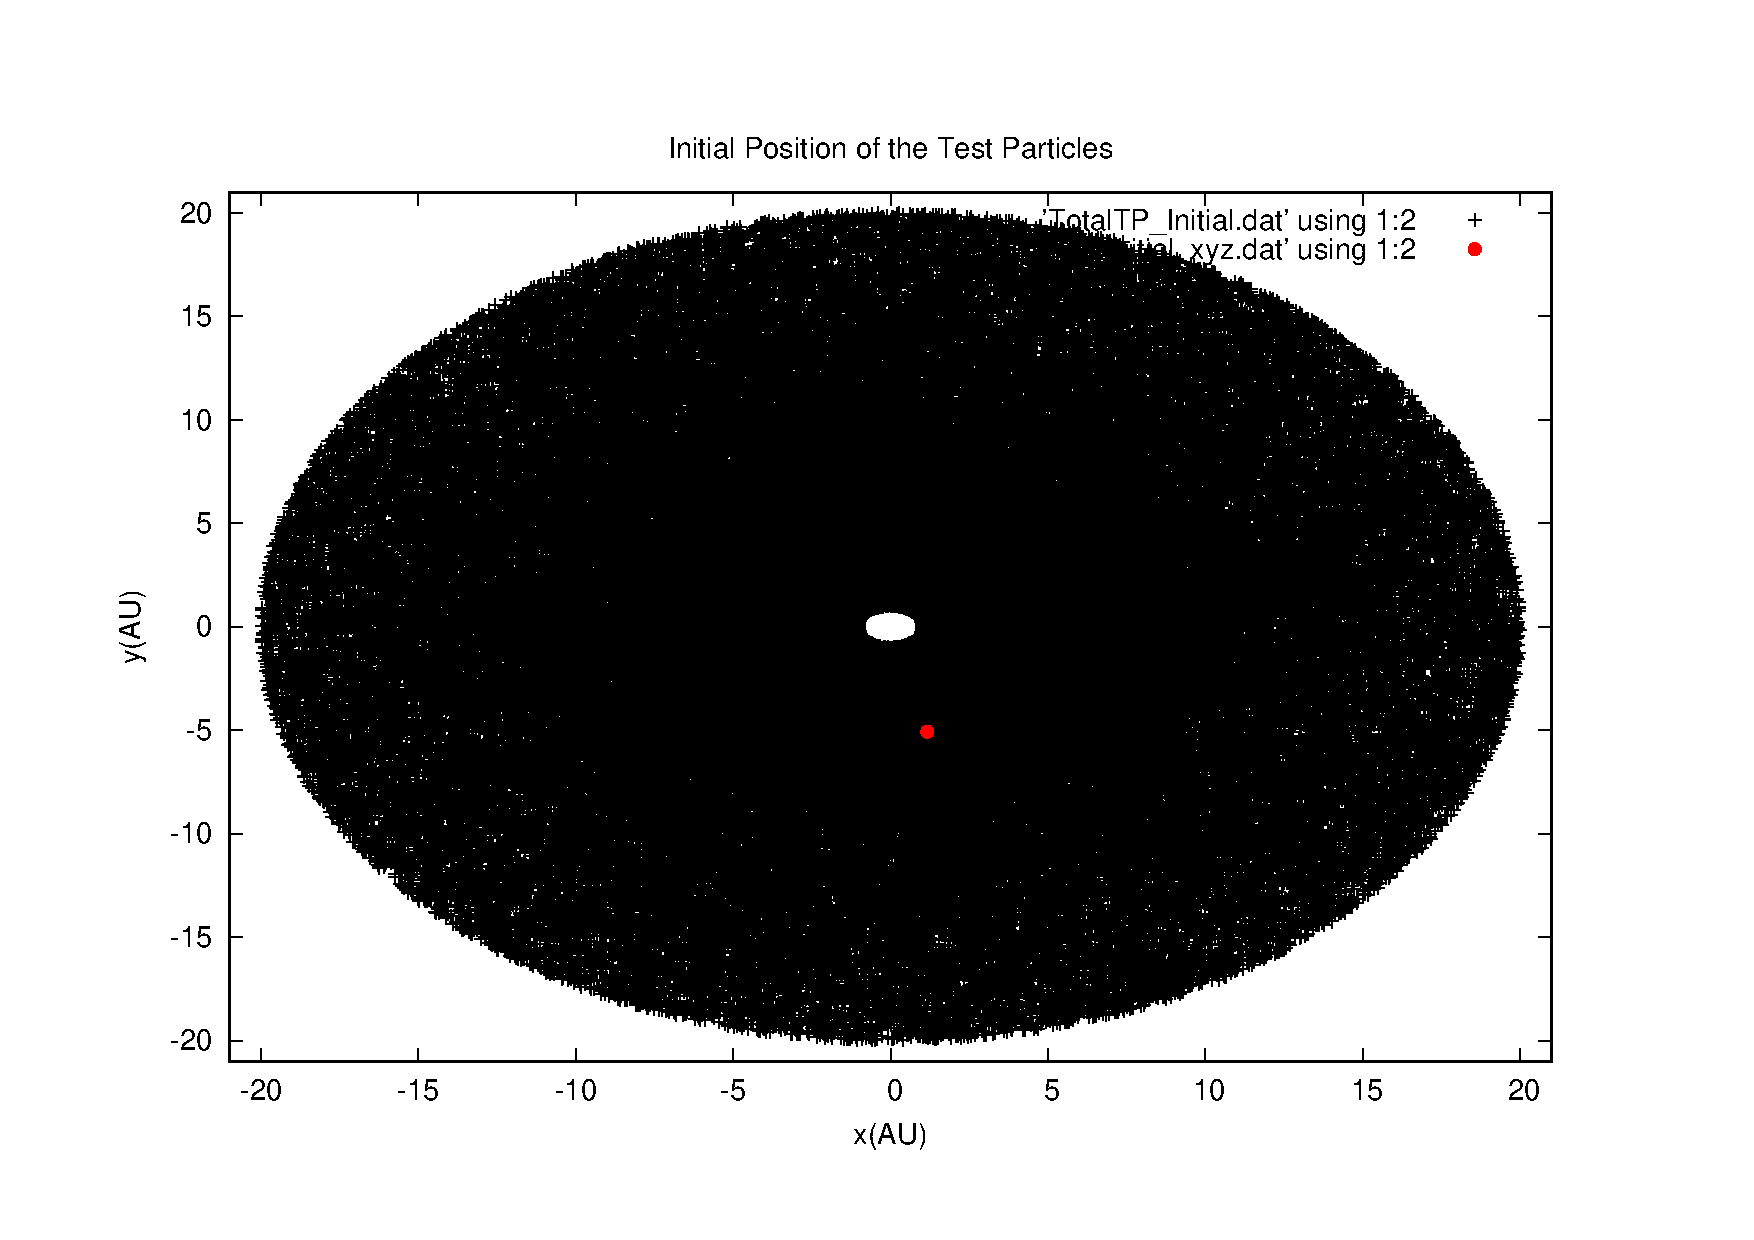
\includegraphics[scale= 0.5]{TotalTP_Initial}
  \caption{Δίσκος της Κατανομής των {\en Test Particles} τη Χρονική Στιγμή {\en $t_0=0 \; sec$ (Initial Disk)}}\label{InitialDisc:figure}
\end{figure}

Η θέση κάθε {\en test particle} στο επίπεδο συμβολίζεται με <<+>> , ενώ η θέση του πλανήτη με <<$\bullet$>>, η οποία στο παρόν γράφημα είναι κόκκινη για να ξεχωρίζει.\\

Λόγω των αρχικών συνθηκών που επιλέξαμε, ο δίσκος παρουσιάζει αξονική και κατοπτρική συμμετρία. Επίσης η {\it αριθμητική του πυκνότητα}, $N_{t_0=0}$, είναι σταθερή και γνωστή $\cdot$ καθώς έχουμε 6000 {\en test particles} σε καθε δακτύλιο πάχους 1 {\en AU}, οπότε μπορούμε να πούμε ότι η {\it επιφανειακή του πυκνότητα}, $\Sigma_{t_0=0}(r)$, μειώνεται συναρτήσει του τετραγώνου της απόστασης καθώς ο ίδιος αριθμός {\en test particles} διαμοιράζεται σε ολοένα και μεγαλύτερου εμβαδού δακτυλίους. Σαν αποτέλεσμα η {\it αριθμητική του πυκνότητα} και κατ' επέκταση η {\it επιφανειακή του πυκνότητα} προσδιορίζονται πλήρως απο τις αρχικές συνθήκες δημιουργίας του δίσκου (αν θεωρήσουμε δεδομένη την μάζα του κάθε {\en test particle}).

\newpage

\section{Παράμετροι της Σκόνης} 

Τα μικρά στερεά σωματίδια αποτελούν την σκόνη και προκειμένου να προσδιορίσουμε τα φυσικά χαρακτηριστικά της καταφύγαμε στις παρακάτω υποθέσεις και παραδοχές:

\begin{itemize}
\item Τα στερεά σωματίδια συγκροτούνται απο το ίδιο υλικό και έχουν ίδια χημική σύσταση, συγκεκριμένα απο $100\%$ πυριτικά άλατα, ({\en Astronomical Silicate}).
\item Τα στερεά σωματίδια θεωρήσαμε ότι είναι συμπαγή και έχουν σφαιρικό σχήμα ακτίνας $r_d$.
\item Τα στερεά σωματίδια χαρακτηρίζονται απο σταθερή πυκνότητα $\rho_d = 2.7 \frac{g}{cm^3}$
\end{itemize}

Οι πληροφορίες σχετικά με την σύσταση του υλικού και την πυκνότητα του πάρθηκαν απο το {\en Database of Optical Constants for Cosmic Dust}, \href{https://www.astro.uni-jena.de/Laboratory/OCDB/index.html}{[{\en OCDB}]}.\\

Στην συγκεκριμένη εργασία κάνουμε λόγο για έναν αρκετά μαζικό δίσκο σχετικά νεαρής ηλικίας και σύμφωνα με την λογική της παραγράφου (1.3.3) επιλέξαμε το μέγεθος των σωματιδίων της σκόνης να είναι λίγο μεγαλύτερο απο αυτό της {\en ISM}. Συνοψίζοντας τα παραπάνω, τα σωματίδια  που επιλέχθηκαν για την παρούσα εργασία είναι:

\begin{table}[h] 
 \centering
 \begin{tabular}{l | l | l | l}
      Ακτίνα ($r_d$) & Πυκνότητα ($\rho_d \; \frac{g}{cm^3}$) & Σύσταση\\
      \hline \hline
     $0.5$ μ$m$ & $2.7$ & $100\%$ πυριτικά άλατα\\
 \end{tabular}
 \caption{Οι Φυσικές Παράμετροι των Σωματιδίων της Σκόνης}\label{tab:ParticlesParameters}
\end{table}   

{\it Το κατώτατο όριο στο μέγεθος δεν είναι τυχαίο καθώς θεωρούμε ότι σωματίδια με ακτίνα $r_{d} < 0.45$ μ$m$ έχουν εκδιωχθεί απο το σύστημα λόγο της πίεσης της ακτινοβολίας του Ήλιου}!\cite{ertel2012observing}\\

Η μάζα του κάθε σωματιδίου ισούται με:

\begin{equation}\label{eq:ParticleMass}
 m=\frac{4 \pi \rho r_d^3 }{3} = 1.41372\times10^{-12} g
\end{equation}

Η συνολική μάζα του δίσκου είναι $M_{disk}= 10^{-4} M_{\odot}=1.99\times10^{29} g$ άρα η μάζα κάθε {\en test particle} είναι:

\begin{equation}\label{eq:InitialTPMass}
 m_{tp}=\frac{10^{-4} M_{\odot}}{114000} = 8.772\times10^{-10} M_{\odot} = 1.746\times10^{24}g
\end{equation}

Απο τις \eqref{eq:ParticleMass} και \eqref{eq:InitialTPMass} το κάθε {\en test particle} αντιπροσωπεύει $N$ σωματίδια, όπου:

\begin{equation}\label{eq:NbParticles}
 N=\frac{m_{tp}}{m}=\frac{1.746\times10^{24}}{1.41372\times10^{-12}} = 1.235\times10^{36}
\end{equation}

Τελικά ο δίσκος την χρονική στιγμή {\en $t_0=0 \; sec$} έχει μάζα $Μ_{disk}=1.99\times10^{29} g$ και περιέχει $N\times114000 = 1.407\times10^{41}$ σωματίδια σκόνης.\\






 